\documentclass{standalone}
\usepackage[utf8]{inputenc}
\usepackage{tikz}
\usepackage{color}
\usetikzlibrary{arrows,shapes,positioning,shadows,trees}

\tikzset{
  basic/.style  = {draw, text width=3cm, drop shadow, font=\sffamily, rectangle},
  root/.style   = {basic, rounded corners=2pt, thin, align=center,
                   fill=white,sibling distance=45mm},
  level 1/.style = {basic, rounded corners=6pt, thin,align=center,
                   text width=10em,sibling distance=80mm},
  level 2/.style = {basic, rounded corners=6pt, thin,align=center,
                   text width=10em,sibling distance=40mm},
  level 3/.style = {basic, rounded corners=6pt, thin,align=center,
                   text width=10em,sibling distance=450mm},
}

\begin{document}

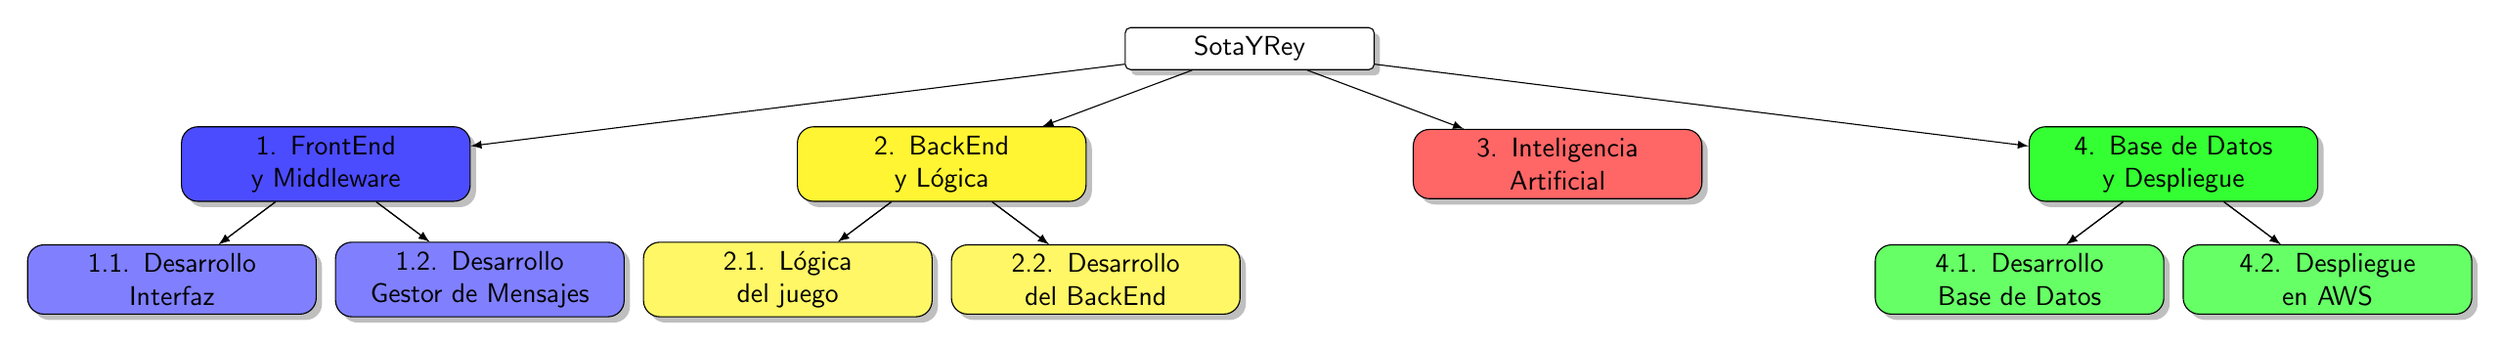
\begin{tikzpicture}[
  edge from parent/.style={->,draw},
  %level 1/.style={sibling distance=45mm},
  %level 2/.style={sibling distance=45mm},
  %level 2/.style={sibling distance=5mm},
  >=latex]

% raiz inicial
\node[root] {SotaYRey}
% The first level, as children of the initial tree
  child {node[level 2, fill=blue!70] (c1) {1. FrontEnd y Middleware}
         child {node[level 3, fill=blue!50] (c11) {1.1. Desarrollo \\ Interfaz}}
        child {node[level 3, fill=blue!50] (c12) {1.2. Desarrollo Gestor de Mensajes}}}
  child {node[level 2, fill=yellow!80] (c2) {2. BackEnd \\ y Lógica}
        child {node[level 3, fill=yellow!60] (c21) {2.1. Lógica \\ del juego}}
        child {node[level 3, fill=yellow!60] (c22) {2.2. Desarrollo del BackEnd \\  }}}
  child {node[level 2, fill=red!60] (c3) {3. Inteligencia \\ Artificial}}
  child {node[level 2, fill=green!80] (c4) {4. Base de Datos \\ y Despliegue}
        child {node[level 3, fill=green!60] (c41) {4.1. Desarrollo Base de Datos}}
        child {node[level 3, fill=green!60] (c42) {4.2. Despliegue \\ en AWS}}};

  

%\begin{scope}
%\node [level 3, below of = c1, node distance=0.5in] (c12) {1.2. Desarrollo Gestor de Mensajes};
%\node [level 3, left of = c12, node distance=1.7in] (c11) {1.1. Desarrollo \\ Interfaz};
%\end{scope}

%\begin{scope}
%\node [level 3, below of = c2, node distance=0.5in] (c21) {2.1. Lógica \\ del juego};
%\node [level 3, right of = c21, node distance=1.7in] (c22) {2.2. BackEnd \\  };
%\end{scope}

%\begin{scope}
%\node [level 3, below of = c4, node distance=0.5in] (c42) {4.2. Despliegue \\ en AWS};
%\node [level 3, left of = c42, node distance=1.7in] (c41) {4.1. Desarrollo Base de Datos};
%\end{scope}

%% The second level, relatively positioned nodes
%\begin{scope}[every node/.style={level 4}]
%\node [below of = c1,node distance=0.5in, xshift=15pt] (c11) {\small{1.1. Diagrama Entidad-Relación} \\ \textcolor{red}{\small{Sergio}}};
%\node [below of = c11, node distance=0.5in] (c12) {\small{1.2. Diseño lógico}\\ \textcolor{red}{\small{Julia}}};
%\node [below of = c12, node distance=0.5in] (c13) {\small{1.3. Implementación tablas (create tables)} \\ \textcolor{red}{\small{Julia}}};

%\node [below of = c21, xshift=30pt] (c211) {\small{2.1.1.UsuarioVO} \\ \textcolor{red}{\small{Julia}}};
%\node [below of = c211] (c212) {\small{2.1.2.StatsUsuarioVO} \\ \textcolor{red}{\small{Julia}}};
%\node [below of = c212] (c213) {\small{2.1.3.PartidaVO} \\ \textcolor{red}{\small{Sergio}}};
%\node [below of = c213] (c214) {\small{2.1.4.LigaVO} \\ \textcolor{red}{\small{Julia}}};
%\node [below of = c214] (c215) {\small{2.1.5.ArticuloVO} \\ \textcolor{red}{\small{Sergio}}};
%\node [below of = c215] (c216) {\small{2.1.6.ArticuloUsuarioVO} \\ \textcolor{red}{\small{Sergio}}};

%\node [below of = c22, xshift=30pt] (c221) {\small{2.2.1.UsuarioDAO} \\ \textcolor{red}{\small{Julia}}};
%\node [below of = c221] (c222) {\small{2.2.2.StatsUsuarioDAO} \\ \textcolor{red}{\small{Julia}}};
%\node [below of = c222] (c223) {\small{2.2.3.PartidaDAO} \\ \textcolor{red}{\small{Sergio}}};
%\node [below of = c223] (c224) {\small{2.2.4.LigaDAO} \\ \textcolor{red}{\small{Julia}}};
%\node [below of = c224] (c225) {\small{2.2.5.ArticuloDAO} \\ \textcolor{red}{\small{Sergio}}};
%\node [below of = c225] (c226) {\small{2.2.6.ArticuloUsuarioDAO} \\ \textcolor{red}{\small{Sergio}}};

%\node [below of = c23, xshift=30pt, node distance = 0.5in] (c231) {\small{2.3.1.Funciones usuario} \\ \tiny{crearUsuario, autentificarUsuario, eliminarUsuario, modificarDatosUsuario, obtenerDatosUsuario, esAdministrador}\\ \textcolor{red}{\small{Julia}}};
%\node [below of = c231, node distance = 0.6in] (c232) {\small{2.3.2.Funciones stats} \\ \tiny{obtenerStatsUsuario, obtenerTodasStatsUsuario} \\ \textcolor{red}{\small{Julia}}};
%\node [below of = c232, node distance = 0.6in] (c233) {\small{2.3.3.Funciones partida} \\ \tiny{crearNuevaPartida, finalizarPartida, obtenerHistorialPartidas, obtenerPartidasPublicasCurso} \\ \textcolor{red}{\small{Sergio}}};
%\node [below of = c233, node distance = 0.65in] (c234) {\small{2.3.4.Funciones liga} \\ \tiny{crearLiga, obtenerDatosLiga, eliminarLiga, modificarDatosLiga, obtenerClasificacionLiga} \\ \textcolor{red}{\small{Julia}}};
%\node [below of = c234, node distance = 0.7in] (c235) {\small{2.3.5.Funciones artículos} \\ \tiny{crearArticulo, eliminarArticulo, modificarArticulo, obtenerArticulo, obtenerArticulosUsuario, comprarArticuloUsuario, obtenerArticulosTienda} \\ \textcolor{red}{\small{Sergio}}};

%\node [below of = c3, xshift=10pt, node distance = 0.5in] (c31) {\small{3.1. Trigger de\\ torneos semanales}\\ \textcolor{red}{\small{Sergio}}};
%\node [below of = c31, node distance=0.6in] (c32) {\small{3.2. Trigger de \\actualización de ligas}\\ \textcolor{red}{\small{Julia}}};
%\end{scope}

\foreach \value in {1,2}
  \draw [->] (c1) edge (c1\value);

\foreach \value in {1,2}
  \draw [->] (c2) edge (c2\value);

\foreach \value in {1,2}
  \draw [->] (c4) edge (c4\value);

%\foreach \value in {1,2,3}
%  \draw[->] (c1.195) |- (c1\value.west);

%\foreach \value in {1,...,6}
%  \draw[->] (c21.195) |- (c21\value.west);

%\foreach \value in {1,...,6}
%  \draw[->] (c22.195) |- (c22\value.west);

%\foreach \value in {1,...,5}
%  \draw[->] (c23.195) |- (c23\value.west);

%\foreach \value in {1,...,2}
%  \draw[->] (c3.195) |- (c3\value.west);

\end{tikzpicture}

\end{document}
